% gjilguid2e.tex
% V2.0 released 1998 December 18
% V2.1 released 2003 October 7 -- Gregor Hutton, updated the web address for the style files.

%\documentclass[extra,mreferee]{gji}
\documentclass[extra]{gji}
\usepackage{timet}

%Extra packages
\usepackage{graphicx}
\usepackage{amsmath}

\title[Gravity anomaly or gravity disturbance?]
      {Should geophysicists use the gravity disturbance or the anomaly?}

\author[Hallam et al.]{
\parbox{\linewidth}{%
    Kristoffer A. T. Hallam$^{1}$\thanks{Emails: kristoffer.hallam@gmail.com, vanderlei@on.br},
    Vanderlei C. Oliveira Jr$^1$,
    Val\'{e}ria C. F. Barbosa$^1$, and \linebreak Leonardo Uieda$^2$
    \vspace{0.3cm}
}%
    \\
    $^1$ Department of Geophysics, Observat\'{o}rio Nacional, Rio de Janeiro, Brazil \\
    $^2$ Department of Geology and Geophysics, SOEST, University of Hawai'i at M\={a}noa, Honolulu, USA
}

\date{Received 2018 Month XX; in original form 2018 Month XX}
\pagerange{\pageref{firstpage}--\pageref{lastpage}}
\volume{XXX}
\pubyear{2018}

%\def\LaTeX{L\kern-.36em\raise.3ex\hbox{{\small A}}\kern-.15em
%    T\kern-.1667em\lower.7ex\hbox{E}\kern-.125emX}
%\def\LATeX{L\kern-.36em\raise.3ex\hbox{{\Large A}}\kern-.15em
%    T\kern-.1667em\lower.7ex\hbox{E}\kern-.125emX}
% Authors with AMS fonts and mssymb.tex can comment out the following
% line to get the correct symbol for Geophysical Journal International.
\let\leqslant=\leq

\newtheorem{theorem}{Theorem}[section]

\newcommand{\versor}[1]{\hat{\mitbf{#1}}}
\renewcommand{\vector}[1]{\vec{\mitbf{#1}}}


\begin{document}

\label{firstpage}

\maketitle


\begin{summary}
 The gravity anomaly is defined as the difference between the Earth's gravity
 on the geoid and the gravity of the normal Earth on the reference ellipsoid.
 Because these quantities are not at the same point, the anomaly contains
 centrifugal accelerations and cannot be considered a harmonic function.
 The gravity disturbance is the difference between gravity and normal gravity
 at the same point.
 Consequently, the centrifugal effects can be neglected and the disturbance can
 be considered a harmonic function.
 This is the premise behind most potential-field data processing techniques
 (e.g., upward/downward continuation and vertical derivatives).
 Unlike the anomaly, the disturbance is due solely to the
 gravitational effects of geologic sources, making it the most appropriate
 for geophysical purposes.
 Use of the gravity anomaly in geophysics carries with it the implicit
 assumption that it is a good approximation for the gravity disturbance.
 However, bear in mind that the difference between the gravity disturbance and
 the free-air anomaly can be larger than 10 mGal worldwide.
 In fact, we argue that the assumptions made during gravity forward and inverse
 modeling imply that the quantity being modelled is the disturbance, not the
 anomaly.
\end{summary}

\begin{keywords}
 potential fields -- gravity disturbance -- gravity anomaly -- gravity modelling.
\end{keywords}


\section{Introduction}

The \textit{gravity vector} is the sum of the gravitational and centrifugal
accelerations felt by a body at rest on the Earth's surface.
Its intensity is what geoscientists call \textit{gravity}
\citep{heiskanen-moritz1967, hofmann-wellenhof-moritz2005}.
When measured on moving platforms (e.g., airplanes,
helicopters, marine vessels), there are additional
non-gravitational accelerations due to the motion of the vehicle,
such as the Coriolis acceleration and high-frequency vibrations
\citep{glennie-etal2000,nabighian-etal2005-grav,baumann-etal2012}.
Geodesists use gravity measurements to estimate the Geoid \citep{li2001}
whereas geophysicists use gravity to estimate the Earth's
internal density distribution.
Hence, geophysicists are usually only interested
in the gravitational component of the observed gravity
because that is what that reflects the Earth's internal density distribution.

The first step toward isolating the gravitational component
is to remove the effects of vehicle motion, Earth tides, instrumental drift,
and barometric pressure changes, among others.
If these effects are properly removed,
the resultant observations are considered to be solely
the sum of the centrifugal acceleration due to the Earth's rotation and
the gravitational acceleration produced by
the internal density distribution of the whole Earth.
The isolation of this particular gravitational component,
and its subsequent use for estimating density
distributions related to geological structures in subsurface,
are the main goals of applied gravimetry \citep{blakely1996}.
The computation of the gravitational effect produced by
the geological structures is known in geophysics as
\textit{gravity modelling}.
Not to be confused with \textit{gravity field modelling}, which
is commonly used in geodesy to denote the mathematical characterization of the
gravity field in local, regional, or global scales (e.g., spherical harmonic
analysis).

We present a discussion of whether the gravity disturbance or the gravity
anomaly should be used in geophysical applications.
The concepts discussed here are well-established in the literature.
However, the debate around this theoretical issue has been
carried about from a more geodetic than a geophysical point of view
\citep{lafehr1991,chapin1996,li2001,fairhead2003,
hackney-featherstone2003,hinze2005}.
We will approach the topic by comparing the geophysical interpretations of the
disturbance and the anomaly.
Our reasoning suggests that the gravity disturbance is more appropriated for
geophysical purposes than the gravity anomaly.


\section{Normal Earth and normal gravity}

The Earth's gravity field is traditionally approximated
by the gravity field of a reference ellipsoid (or level ellipsoid).
This model is rigid and geocentric,
with a minor axis $b$ which coincides with
the mean rotation axis of the Earth $Z$.
The ellipsoid has the same total mass as the Earth (including the atmosphere)
and also the same angular velocity \citep{heiskanen-moritz1967,
vanicek1987,hofmann-wellenhof-moritz2005,torge2012}.
Its limiting surface coincides with
a particular equipotential of its own gravity field.
Here, we follow \citep{torge2012} and call this reference ellipsoid
the \textit{normal Earth}.
Analogously to the Earth, the \textit{normal gravity vector} is
the sum of the
gravitational and centrifugal accelerations exerted by the normal
Earth on a body at rest at a point $P$.
The intensity of the normal gravity vector is called \textit{normal gravity}.

It is worth noting that, although the normal Earth has the same total mass as
the Earth, its internal density distribution is left unspecified.
The search for geologically meaningful density distributions
for the interior of the normal Earth has
geophysical rather than geodetic motives \citep{marussi1974}.
In physical geodesy, a model for the normal gravity field
can be arbitrarily defined with the sole purpose of
keeping the difference from the actual gravity field
as small as possible \citep{vanicek1987}.
The only condition imposed on its internal density
distribution is that it produces a gravity field
having a particular equipotential which coincides
with its limiting surface.


\section{Terrestrial Reference Systems used in gravity modelling}

For geophysical gravity modelling purposes, there are three important
Terrestrial Reference Systems.
They rotate with the Earth and are used for describing
positions and movements of objects on and close to the Earth's surface
\citep{torge2012}.

The first is a geocentric system of Cartesian coordinates
having the $Z$-axis coincident with the mean rotational axis of the Earth,
the $X$-axis pointing to the Greenwich meridian,
and the $Y$-axis completing a right-handed system (Fig. \ref{fig:GCS-GGS}).
This reference system is called by different names in the literature:
Mean Terrestrial System \citep[e.g.,][]{soler1976},
Earth-fixed geocentric Cartesian system \citep[e.g.,][]{torge2012}
or Earth-centered Earth-fixed system \citep[e.g.,][]{bouman_etal2013},
for example.
Here, we opted for using the term Geocentric Cartesian System (GCS).

The second is a geocentric system of geodetic coordinates
(the Geocentric Geodetic System or GGS),
which is defined by the reference ellipsoid used as the Normal Earth
\citep{heiskanen-moritz1967, soler1976, torge2012, bouman_etal2013}.
The position of a point is defined by
the \textit{geometric height} $h$,
the \textit{geodetic latitude} $\varphi$,
and the \textit{longitude} $\lambda$ (Fig. \ref{fig:GCS-GGS}).
There are also three mutually-orthogonal unit vectors defined at a given point
\citep{soler1976}:

\begin{equation}
    \versor{u} =
    \begin{bmatrix}
        \cos\varphi \, \cos\lambda \\
        \cos\varphi \, \sin\lambda \\
        \sin\varphi
    \end{bmatrix}
    \versor{v} =
        \begin{bmatrix}
        -\sin\varphi \, \cos\lambda \\
        -\sin\varphi \, \sin\lambda \\
        \cos\varphi
    \end{bmatrix}
    \versor{w} =
    \begin{bmatrix}
        -\sin\lambda \\
        \cos\lambda \\
        0
    \end{bmatrix} .
    \label{eq:unit-vectors}
\end{equation}

\noindent Equations for converting between these systems can be found in
the literature \citep[e.g.,][]{heiskanen-moritz1967, torge2012,
bouman_etal2013}.

The third is the Topocentric Cartesian System (TCS),
which is commonly used in local or regional scale geophysical studies.
The origin of the TCS is located at a point $P$,
axes $x$ and $y$ are parallel to
the unit vectors $\versor{v}$ and $\versor{w}$
(eq. \ref{eq:unit-vectors}), respectively,
and the $z$-axis is opposite to the unit vector $\versor{u}$
(Fig. \ref{fig:TCS}).


\section{gravity disturbance and gravity anomaly}

Let $\vector{\gamma}_{P}$ and $\vector{g}_{P}$ and be, respectively,
the \textit{normal gravity vector} and the Earth's \textit{gravity vector}
(corrected from non-gravitational effects due to vehicle
motion and time variations such as Earth tides and instrumental drift),
both located at a point $P$.
In this case, the gravity vector $\vector{g}_{P}$ is the
gradient of the scalar \textit{gravity potential},
which is the sum of a gravitational potential and a centrifugal potential.
Similarly, the normal gravity vector $\vector{\gamma}_{P}$ is the
gradient of the scalar \textit{normal potential},
which is also the sum of a gravitational and a centrifugal potential.
By definition, the centrifugal part of
the normal potential and the gravity potential are equal.

The difference between $\vector{g}_{P}$ and $\vector{\gamma}_{P}$,
which we emphasize are located at the same point $P$,
is the \textit{gravity disturbance vector} (Fig. \ref{fig:surfaces}):

\begin{equation}
\delta \vector{g}_{P} =
\vector{g}_{P} - \vector{\gamma}_{P} \: .
\label{eq:gravity-disturbance-vector}
\end{equation}

Because the centrifugal parts of both the normal gravity vector
and the Earth's gravity vector are equal,
the gravity disturbance vector $\delta \vector{g}_{P}$
represents a purely gravitational effect.
As a consequence of the superposition principal \citep{blakely1996},
this effect is caused by contrasts between
the internal density distributions
of the actual Earth and the normal Earth.
In applied geophysics, these density differences are generally called
\textit{anomalous masses} \citep[e.g.,][]{hammer1945,lafehr1965},
\textit{density anomalies} \citep[e.g.,][]{forsberg1984},
or \textit{gravity sources} \citep[e.g.,][]{blakely1996}.
Here, we opted for using the last term.

The difference between the magnitudes of the gravity vector
$g_{P} = \| \vector{g}_{P} \|$ and the normal gravity vector
$\gamma_{P} = \| \vector{\gamma}_{P} \|$,
at the same point $P$, is the \textit{gravity disturbance}
\citep{heiskanen-moritz1967, hofmann-wellenhof-moritz2005}:

\begin{equation}
\delta g_{P} = g_{P} - \gamma_{P} \: .
\label{eq:gravity-disturbance}
\end{equation}

\noindent
Notice that $\delta g_{P}$ is not equivalent
to the magnitude of the gravity disturbance vector
$\delta \vector{g}_{P}$ \citep{barthelmes2013, sanso_sideris2013}.

The \textit{gravity anomaly vector}
is the difference between the gravity
vector at a point $Q^{\prime}$ on the geoid
(a particular equipotential surface of the gravity potential)
and the normal gravity vector at a point $Q$ on the surface of the ellipsoid,
both located at the same geodetic latitude and longitude
(Fig. \ref{fig:surfaces}):

\begin{equation}
\Delta \vector{g} = \vector{g}_{Q^{\prime}} - \vector{\gamma}_{Q} .
\label{eq:gravity-anomaly-vector}
\end{equation}

Similarly to the gravity disturbance (eq. \ref{eq:gravity-disturbance}),
the \textit{gravity anomaly} is given by

\begin{equation}
\Delta g = g_{Q^{\prime}} - \gamma_{Q} ,
\label{eq:gravity-anomaly}
\end{equation}

\noindent
where $g_{Q^{\prime}}$ is the magnitude of the gravity vector on the geoid,
and $\gamma_{Q}$ is the magnitude of the normal gravity vector
on the reference ellipsoid (Fig. \ref{fig:surfaces}).

The gravity anomaly is not defined at a particular point.
Instead, as properly pointed out by \citet{barthelmes2013},
it depends only on longitude and latitude and is not a function of height.
Because gravity and normal gravity are located at different points,
the gravity anomaly is a combination of gravitational and centrifugal effects,
rather than purely gravitational effects like the gravity disturbance.
Consequently, its upward continuation, for example, cannot be rigorously done
because it is not a harmonic function.
However, upward continuation of gravity anomalies is commonly seen in the
literature.
In doing so, an implicit assumption is being made that the gravity anomaly is
an approximation of the gravity disturbance,
which in turn can be represented by a harmonic function and can be upward
continued.

Different approximations for the gravity anomaly can be calculated
depending on the corrections applied to them.
These corrections are usually called \textit{gravity reductions}.
The \textit{free-air anomaly}, for example, can be defined as
\citep{blakely1996, hofmann-wellenhof-moritz2005}:

\begin{equation}
\Delta g^{F} = g_{P}
- \gamma_{Q} - \frac{\partial \gamma}{\partial h} \, H_{P} \: ,
\label{eq:free-air-anomaly}
\end{equation}

\noindent
where the rightmost term is called the \textit{free-air correction},
$\partial \gamma/\partial h \approx -0.3086$ mGal/m is the
derivative of the normal gravity with respect to the geometric height $h$,
and $H_{P}$ is the orthometric height (i.e., with respect to the geoid)
of point $P$ (Fig. \ref{fig:surfaces}).
The free-air correction can be interpreted as a downward continuation of
$g_P$ to the geoid or as an upward continuation of $\gamma_Q$ to a height
$H_P$.
Regardless, we can also apply the free-air correction
to calculate the gravity disturbance by
approximating the normal gravity $\gamma_{P}$
at a point $P$ on the Earth's surface
from the normal gravity at the ellipsoid $\gamma_{Q}$:

\begin{equation}
\delta g_{P} \approx g_{P} -
\left( \gamma_{Q} + \frac{\partial \gamma}{\partial h} h_P \right) \: .
\label{eq:gravity-disturbance-approx}
\end{equation}

\noindent
where $h_P$ is the geometric height of point P.
However, using the free-air correction to calculate the disturbance is
discouraged because an analytical expression exists for calculating $\gamma$ at
any point on or above the ellipsoid \citep{li2001}.

Using eqs. \ref{eq:free-air-anomaly} and \ref{eq:gravity-disturbance-approx},
we can estimate the absolute difference between the gravity disturbance and the
free-air anomaly:

\begin{equation}
\left\vert \delta g_{P} - \Delta g^{F} \right\vert \approx
\left\vert \frac{\partial \gamma}{\partial h} N \right\vert \: ,
\label{eq:difference-disturbance-free-air}
\end{equation}

\noindent
where $N \approx h - H$ is the geoidal height (Fig. \ref{fig:surfaces}).
This approximation assumes that the geoid and the surface of
the reference ellipsoid are close to being parallel at $P$
and the surrounding area.
Eqs \ref{eq:gravity-disturbance-approx}
and \ref{eq:difference-disturbance-free-air} are commonly used
in geodesy to define the \textit{fundamental equation of physical
geodesy} \citep{hofmann-wellenhof-moritz2005}.

We know empirically that $N$ is $\approx \pm 1$ m on the oceans
and reaches a maximum absolute value of $\approx 120$ m
\citep[e.g.,][]{torge2012, sanso_sideris2013}.
In Brazil, for example, the geoidal height
varies between $\approx \pm 30$ m \citep{ibge_mapgeo2015}.
Consequently,
the maximum absolute difference between the gravity disturbance and
the free-air anomaly in Brazil,
according to eq. \ref{eq:difference-disturbance-free-air},
is $\approx 9.258$ mGal.


\section{The effect of topographic masses}

The \textit{Bouguer correction} can be applied to the free-air anomaly
to remove the gravitational effect of the topographic masses
between the observation point $P$ and the point on the geoid $Q^\prime$.
The \textit{Bouguer anomaly} is defined in the continents as
\citep{blakely1996, hofmann-wellenhof-moritz2005}:

\begin{equation}
\Delta g^{B} = g_{P}
    - \gamma_{Q}
    - \frac{\partial \gamma}{\partial h} \, H_{P}
    - 2 \pi G \rho_{t} \, H_{P}
     \: ,
\label{eq:simple-bouguer-anomaly}
\end{equation}

\noindent
where $\rho_t$ is the density of the topographic masses and $G$ is the
gravitational constant.
Th Bouguer correction approximates the gravitational effect that all
topographic masses above the geoid exert on point $P$ by the effect of a
homogeneous, infinitely extended slab of constant density $\rho_{t}$ and
thickness $H_{P}$.
A similar correction can be applied to the gravity disturbance
(using the approximation in eq. \ref{eq:gravity-disturbance-approx})
to remove the effect of topographic masses between
the observation point $P$ and a point on the ellipsoid $Q$.
We will call this quantity the \textit{Bouguer disturbance}:

\begin{equation}
\delta g_P^{B} \approx
g_{P} -
\left( \gamma_{Q} + \frac{\partial \gamma}{\partial h} h_P \right)
- 2 \pi G \rho_{t} \, h_{P} \: .
\label{eq:bouguer-disturbance}
\end{equation}

At first glance, the only difference between eqs.
\ref{eq:simple-bouguer-anomaly} and \ref{eq:bouguer-disturbance} is the use of
orthometric ($H_P$) versus geometric ($h_P$) heights.
However, their geophysical interpretations are significantly different.
Apart from the centrifugal effect mentioned in the previous section,
the Bouguer anomaly (eq. \ref{eq:simple-bouguer-anomaly}) still contains
the gravitational effect of topographic masses between the geoid and ellipsoid.
Conversely, when calculating the Bouguer disturbance one removes the effects of
an ellipsoidal reference model (the normal Earth) and the known topographic
masses between the surface of the ellipsoid and observation point.
Hence, the Bouguer disturbance can be interpreted as being solely the
gravitational effect produced by the density contrasts between the actual
internal density distribution of the Earth and that of the normal Earth plus a
homogeneous topography.

There was a certain lack of comprehension regarding the geophysical meaning of
gravity anomalies until the mid 90s.
As properly pointed out by \citet{chapin1996},
``although the corrections which bring about a Bouguer gravity anomaly are well
established, the reasons for doing them are not well understood. One cause of
this common misunderstanding is that the subject has been poorly presented in
many of the basic texts''.
In his seminal book, \citet{blakely1996} shed some light on the geophysical
meaning of gravity anomalies from the perspective of applied geophysics and
their relationship to the gravity sources.
We complement this interpretation by stressing the fact that
gravity anomalies reflect not only the gravity sources,
but also a combination of gravitational and centrifugal effects.
These additional, non-harmonic and undesired effects are due to the calculation
of the normal gravity at a point other than that were gravity is measured.


\section{Gravity modelling}

We have established that the gravity disturbance is due solely to the
gravitational effect of the gravity sources.
Now we will discuss how this relates to some assumptions made during gravity
modelling.

The gravity vector $\vector{g}_i$ (eq. \ref{eq:gravity-disturbance-vector})
at a point $(x_i, y_i, z_i)$ in the TCS (Fig. \ref{fig:TCS}a) can be
represented by:

\begin{equation}
\vector{g}_i = \vector{\gamma}_i + \delta \vector{g}_i \: .
\label{eq:gravity-vector-TCS}
\end{equation}

\noindent
Furthermore, the gravity $g_i$ can be approximated by a first order Taylor's
expansion \citep{sanso_sideris2013}:

\begin{equation}
g_i \approx \gamma_i +
\versor{\gamma}_i^{\top} \delta \vector{g}_i \: ,
\label{eq:gobs-approx}
\end{equation}

\noindent
where $^{\top}$ denotes transposition and $\versor{\gamma}_{i}$ is a unit
vector with the direction of the normal gravity vector.
This approximation is valid because
$\gamma_{i} \gg \| \delta \mathbf{g}_{i} \|$ at all points on or above the
Earth's surface.
It is known in geodesy \citep[e.g.,][]{sanso_sideris2013}
and is analogous to the approximation used for
total-field magnetic anomalies \citep[e.g.,][]{blakely1996}.
In local or regional scales, the unit
vector $\versor{\gamma}_{i}$
may be considered constant throughout the study area and
parallel to the $z$ axis of the TCS (Fig. \ref{fig:TCS}a).

Using eq. \ref{eq:gobs-approx} and fixing $\gamma$ at a point $P$ at
the origin of the TCS (Fig. \ref{fig:TCS}a),
the gravity disturbance can be rewritten as:

\begin{equation}
\delta g_{i} \approx \versor{\gamma}_{P}^{\top} \delta \vector{g}_{i} \: .
\label{eq:gravity-disturbance-approx-TCS}
\end{equation}

\noindent
This equation shows that the gravity disturbance $\delta g_{i}$ is
approximately the component of the $\delta \vector{g}_{i}$ in the direction of
the normal gravity vector $\vector{\gamma}_P$
\citep{hofmann-wellenhof-moritz2005, sanso_sideris2013}.
Because $z$-axis of the TCS is parallel to $\vector{\gamma}_P$
(Fig. \ref{fig:TCS}b), the gravity disturbance can be defined as the
$z$-component of the gravitational attraction exerted by the gravity sources at
the point $(x_{i}, y_{i}, z_{i})$.
As a consequence, the gravity disturbance can be modelled by the harmonic
function:

\begin{equation}
d_{i} = \iiint\limits_{v}
\frac{G \, \Delta\rho(x^{\prime}, y^{\prime}, z^{\prime}) \,
[z_{i} - z^{\prime}]}
{\sqrt{[x_{i} - x^{\prime}]^{2} +
[y_{i} - y^{\prime}]^{2} + [z_{i} - z^{\prime}]^{2}}} \: dv^{\prime} \: ,
\label{eq:gz-local}
\end{equation}

\noindent
where $\Delta\rho(x^{\prime}, y^{\prime}, z^{\prime})$
is the density contrast at a point $(x^{\prime}, y^{\prime}, z^{\prime})$
within the volume $v$ and the integration is conducted over $x^{\prime}$,
$y^{\prime}$ and $z^{\prime}$.

In practice, most instances of gravity modelling in the literature use Bouguer
anomalies and function $d_{i}$ (usually presented as ``$g_z$'') to represent
the gravitational effect of gravity sources.
Consequently, these studies are using the gravity
anomaly as an approximation for the gravity disturbance.
Notice that $d_{i}$ does not depend on the
height with respect to the geoid (orthometric height).
Rather, it depends on the relative position of the gravity sources and the
observation point $(x_{i}, y_{i}, z_{i})$ in the TCS (Fig. \ref{fig:TCS}a).
Finally, it is important to mention that gravimeters do not measure $d_{i}$ but
$\| \vector{g}_i \|$.


\section{Conclusions}

Although the gravity disturbance is well-known in geodesy,
its use in applied geophysics is uncommon.
For years, geophysicists have been using gravity anomalies for modelling
the gravitational effects of geological bodies.
Wether geophysicists should use the gravity anomaly or the gravity disturbance
is of more than mere academic interest.
It is a question that underpins the very assumptions about what it is that we
are actually modelling.

The gravity anomaly is the difference between
gravity on the geoid and normal gravity on the reference ellipsoid.
The gravity disturbance is the difference between gravity and normal gravity at
the same point.
Because of this, the gravity disturbance is a purely gravitational effect,
whereas the gravity anomaly is a combination of gravitational and centrifugal
effects.
Consequently, the gravity disturbance is a harmonic function while the
gravity anomaly is not.
Being a harmonic function is the premise required by most techniques for
processing potential-field data
(e.g., upward/downward continuation, operations with the equivalent layer,
conversions between gravity and magnetic data, computation of vertical
derivatives).
Hence, the gravity disturbance is the logical choice for
representing the gravitational effects produced by the heterogeneous density
distribution of the Earth.

More often than not, gravity modelling is done by computing the
vertical component of the gravitational acceleration exerted by the sources.
We have shown that, in doing so, one is actually computing the gravity
disturbance while attempting to fit a gravity anomaly.
This is a clear inconsistency.
Doing so may even result in wrong interpretations of a quantitative nature.
In Brazil, for example, the maximum difference
between the gravity disturbance and the free-air anomaly reaches 9 mGal.
Such difference at the Earth's surface may lead to
an error of XXX m in the depth-to-center estimate of a sphere with
true depth-to-center at xxx m, radius xxxx m, and density
contrast of xxx $kg.m^{-3}$.

In practice, most of these issues can be nullified during data processing by
substituting orthometric heights (i.e., with respect to the geoid) with
geometric heights (i.e., with respect to the ellipsoid).
For modern acquisitions, this requires no extra work because GPS already
provide geometric heights.
The free-air correction can even be bypassed entirely by computing $\gamma_P$
directly.
As a bonus, the gravity disturbance is conceptually simpler to understand and
doesn't require the concept of the geoid with which learners often struggle.


\begin{acknowledgments}
The authors would like to thank the editor and all the
reviewers for their criticisms and corrections.
\end{acknowledgments}

\bibliographystyle{gji}
\bibliography{bib-file}


\appendix
%\section{For authors}
%
%Table~\ref{authors} is a list of design macros which are unique to GJI. The
%list displays each macro's name and description.
%
%\section{For editors}
%
%The additional features shown in Table~\ref{editors} may be used for
%production purposes.
%
%\bsp % ``This paper has been produced using the Blackwell
%     %   Publishing GJI \LaTeXe\ class file.''

\begin{figure}
%    \vspace{5.5cm}
    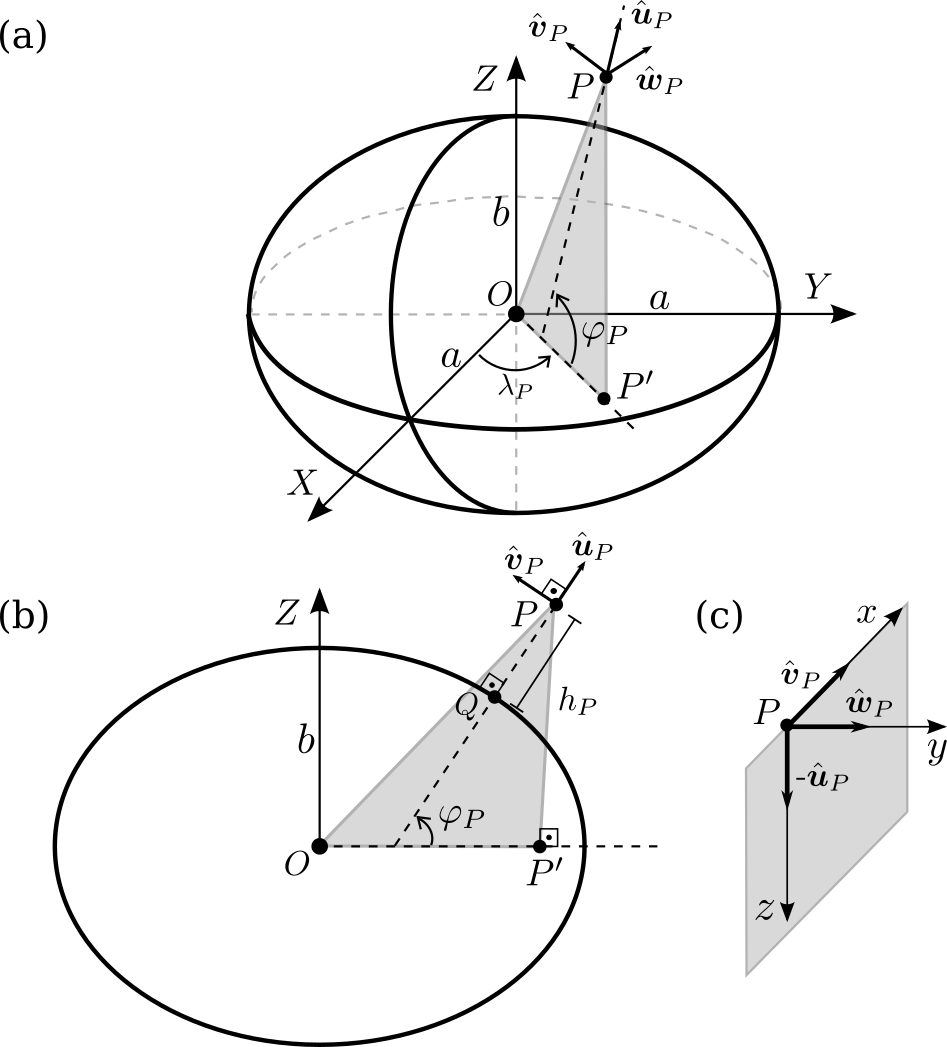
\includegraphics{figures/cartesian-geodetic-systems.png}
    \caption{
    The Geocentric Cartesian System (GCS) and the Geocentric Geodetic System
    (GGS).
    The GGS is defined by an oblate ellipsoid with semi-minor axis $b$ and
    semi-major axis $a$.
    In this coordinate system, the position of a point is determined by the
    geometric height $h$, geodetic latitude $\varphi$, and longitude $\lambda$.
    $O$ is the Earth's center of mass, $P$ is an observation point, and
    unit vectors $\versor{u}$, $\versor{v}$, and $\versor{w}$ define mutually
    orthogonal directions at $P$ (eq. \ref{eq:unit-vectors}).
    In (b), $Q$ is the projection of $P$ onto the reference ellipsoid at
    the same latitude and longitude.
    }
  \label{fig:GCS-GGS}
\end{figure}

\begin{figure}
    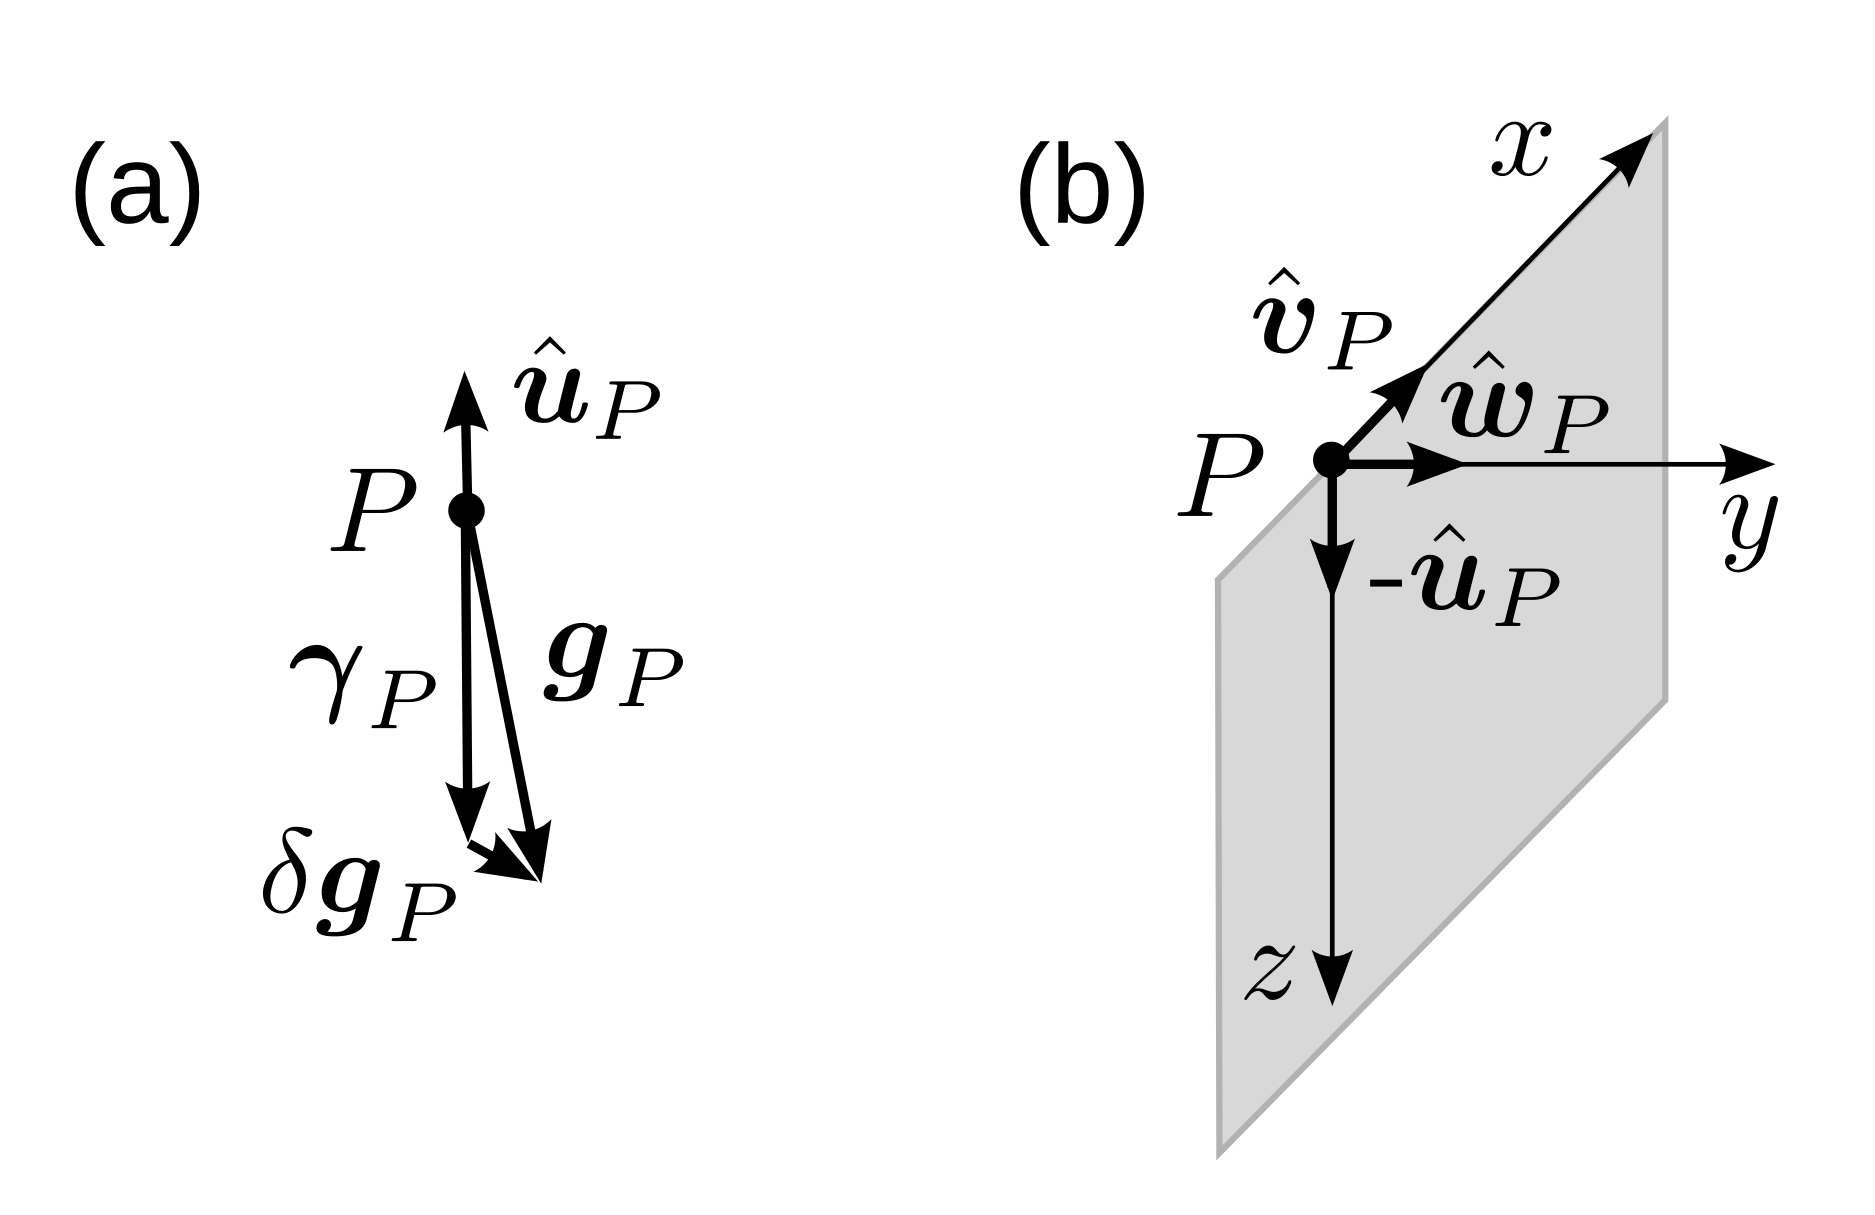
\includegraphics{figures/local-system.png}
    \caption{
    (a) The topocentric Cartesian coordinate system (TCS) with origin at a
    point $P$.
    Axes $x$ and $y$ are parallel to the unit vectors $\versor{v}$ and
    $\versor{w}$ (eq. \ref{eq:unit-vectors} and Fig. \ref{fig:GCS-GGS}),
    respectively, and the $z$ axis is opposite to $\versor{u}$.
    The gray plane is the same shown in Fig. \ref{fig:GCS-GGS}.
    (b) Schematic representation of the gravity vector
    $\vector{g}_{P}$, normal gravity vector $\vector{\gamma}_{P}$,
    gravity disturbance vector $\delta \vector{g}_{P}$
    (eq. \ref{eq:gravity-disturbance-vector}) and unit vector
    $\versor{u}_{P}$ (eq. \ref{eq:unit-vectors}) at a point
    $P$.
    }
  \label{fig:TCS}
\end{figure}

\begin{figure}
    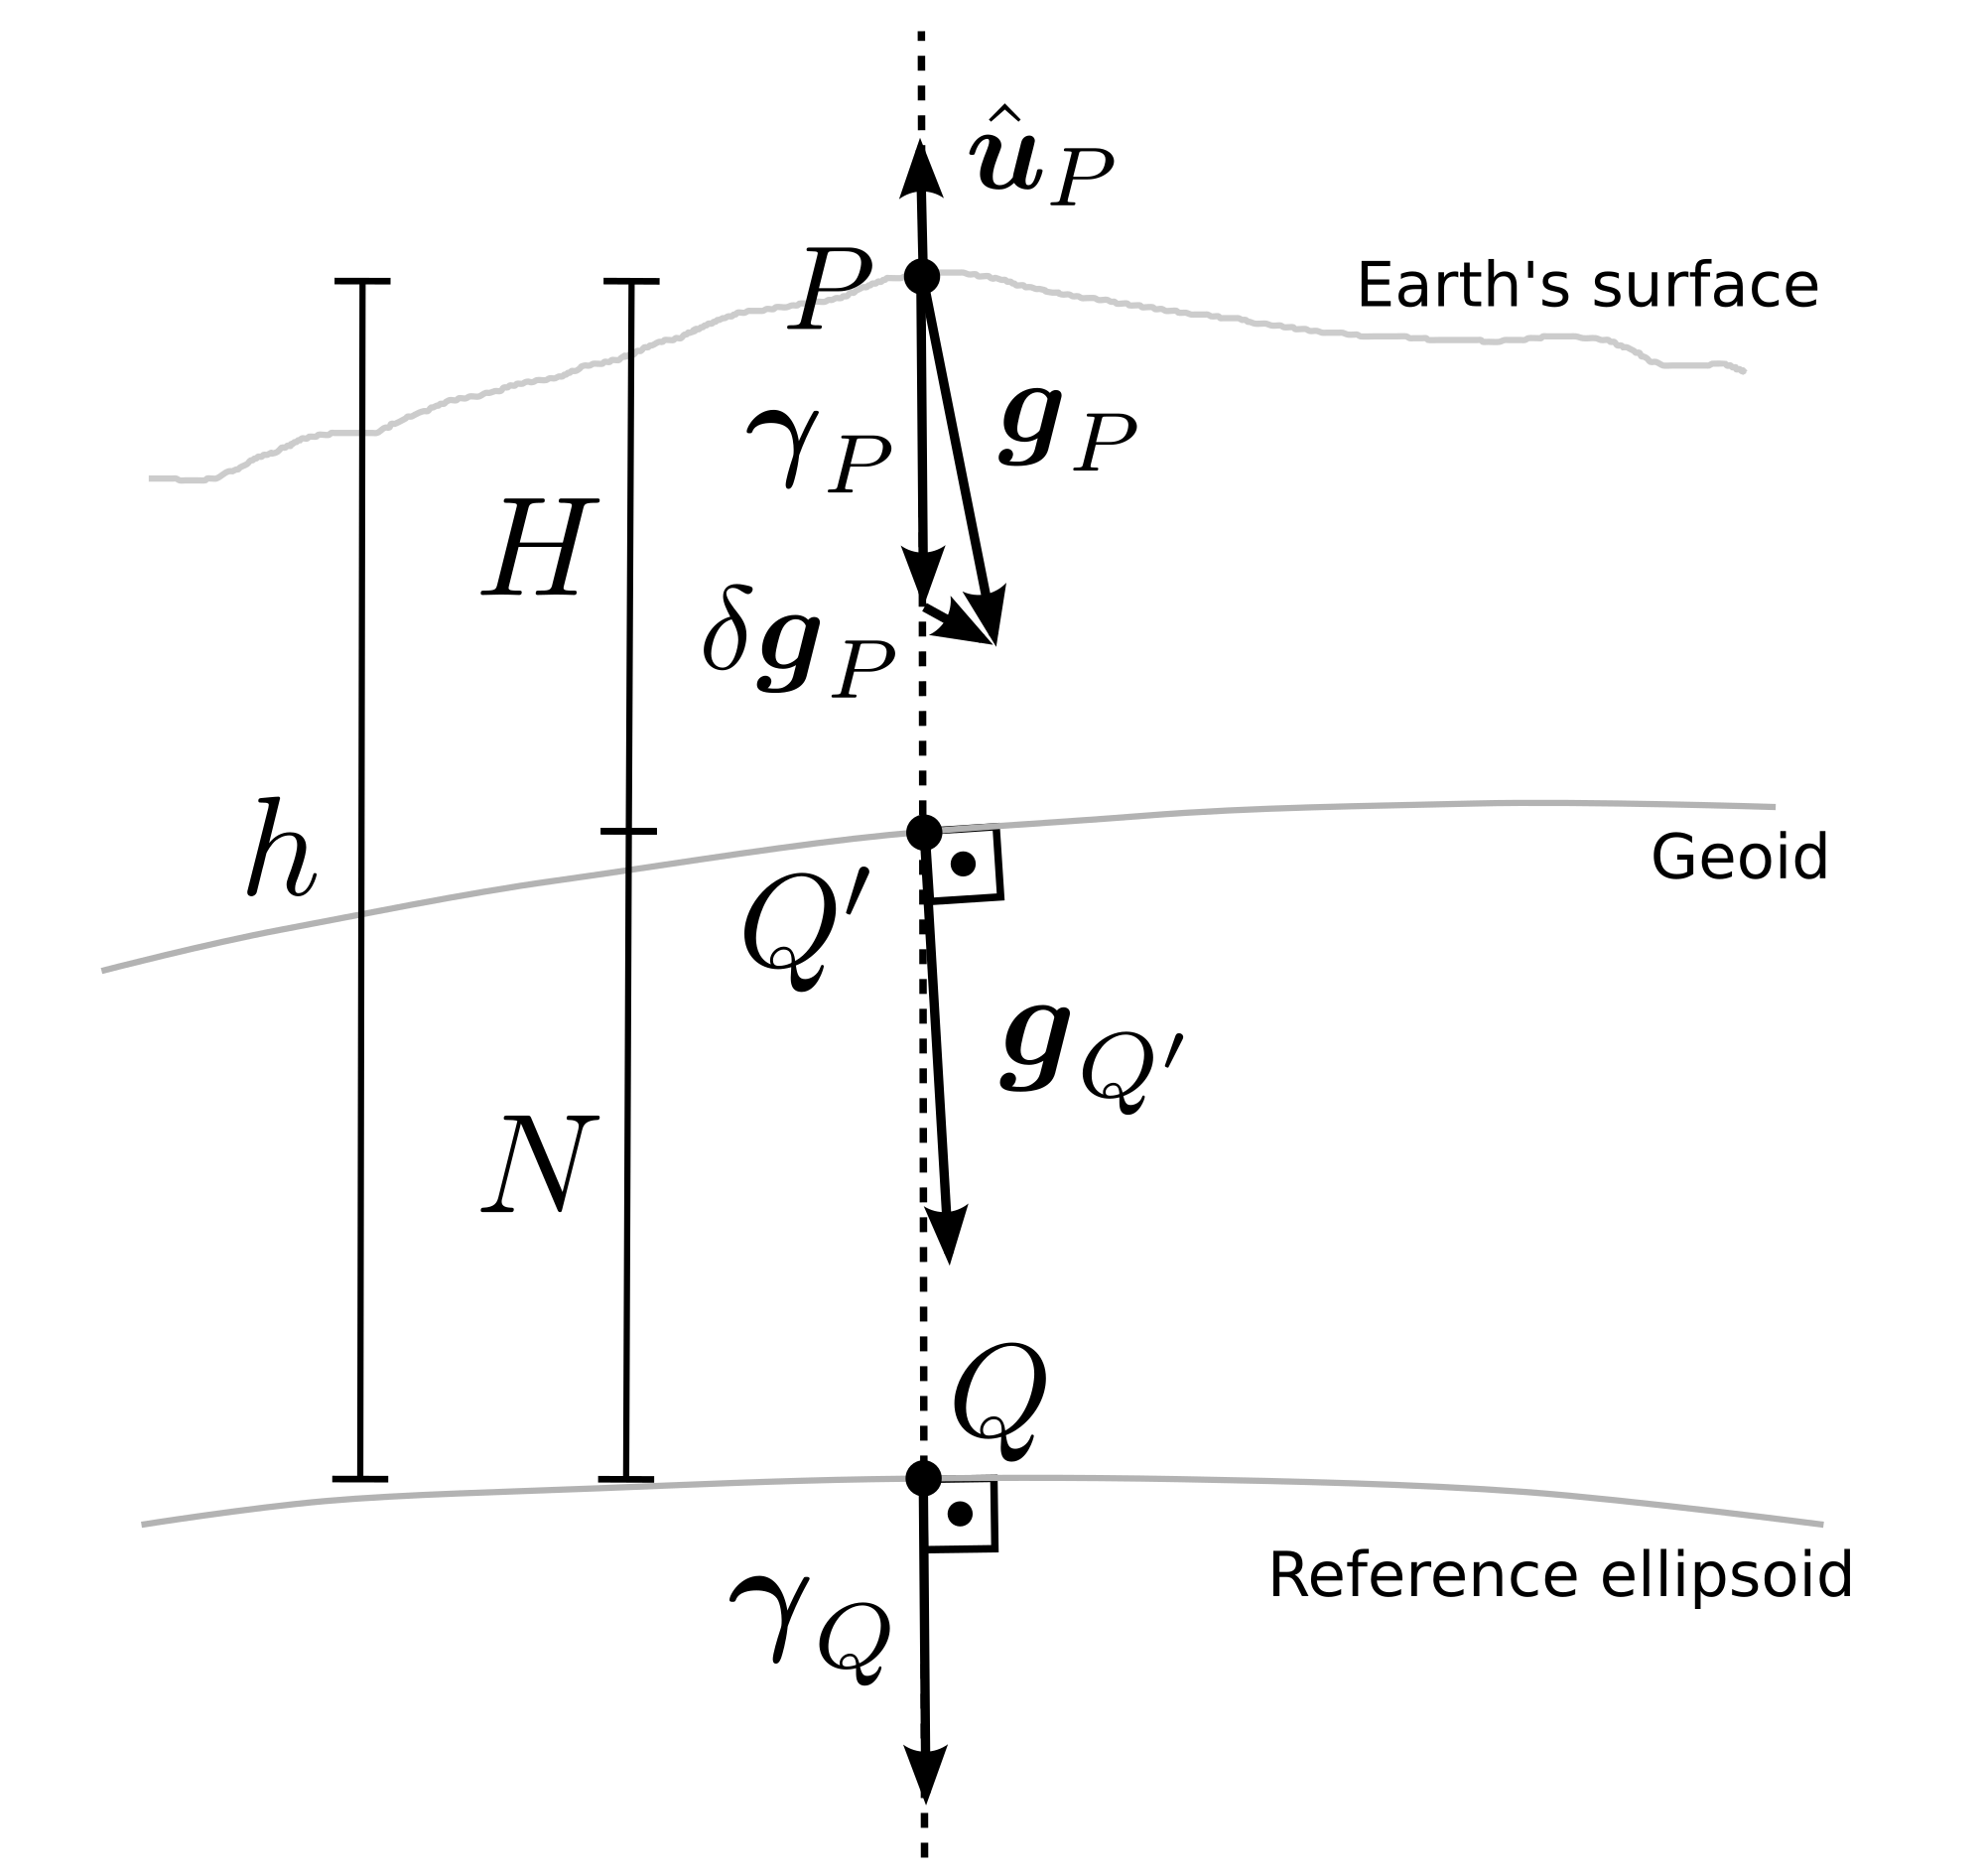
\includegraphics{figures/surfaces.png}
    \caption{
    The gravity vector
    $\vector{g}_{P}$, normal gravity vector $\vector{\gamma}_{P}$,
    gravity disturbance vector $\delta \vector{g}_{P}$
    (eq. \ref{eq:gravity-disturbance-vector}), and unit vector
    $\versor{u}_{P}$ (eq. \ref{eq:unit-vectors}) at a point $P$
    on the surface of the Earth.
    The gravity vector $\vector{g}_{Q^{\prime}}$
    at a point $Q^{\prime}$ on the geoid, normal gravity vector
    $\vector{\gamma}_{Q}$ at a point $Q$ on the reference ellipsoid,
    geometric height $h$, orthometric height $H$, and geoidal height $N$.
    The dashed line passing through
    $Q$, $Q^{\prime}$ and $P$ is normal to the
    surface of the reference ellipsoid at $Q$.
    This figure shows a commonly used approximation in which the ellipsoid and
    geoid are represented as parallel surfaces so that $h \approx H + N$.
    }
  \label{fig:surfaces}
\end{figure}

\label{lastpage}


\end{document}
